\documentclass[a4paper,twoside,11pt]{article}
\usepackage{a4wide,graphicx,fancyhdr,amsmath,amssymb,float, caption, hyperref}
\usepackage{listings}

%----------------------- Macros and Definitions --------------------------

\setlength\headheight{20pt}
\addtolength\topmargin{-10pt}
\addtolength\footskip{20pt}

\newcommand{\R}{{\mathbb R}}
\newcommand{\dir}{\vec{d}}
\newcommand{\pol}{{\cal P}}
\newcommand{\robot}{{\cal R}}
\newcommand{\triang}{{\cal T}}
\newcommand{\dist}{\mathrm{dist}}
\newcommand{\eps}{\varepsilon}
\newcommand{\Mid}{:}
\newcommand{\ch}{\mathcal{CH}}
\newcommand{\exercise}[1]{\noindent{\bf Exercise #1:}}
\newenvironment{solution}{\begingroup\Solenv}{\END\endgroup}
\def\Solenv{\vspace{.5\baselineskip}\penalty100\advance\leftskip by\parindent
  \advance\leftmargini by\parindent
  \Sol\ \ignorespaces}
\def\Sol{\noindent{\bf Solution\/:}\nobreak}
\def\END{\unskip~\medbreak\medbreak\medbreak}
\def\qed{\hfill$\Box$}

\newtheorem{theorem}{Theorem}
\newtheorem{lemma}[theorem]{Lemma}

\fancypagestyle{plain}{%
\fancyhf{}
\fancyhead[LO,RE]{\sffamily Eindhoven University of Technology}
\fancyhead[RO,LE]{\sffamily }
\fancyfoot[LO,RE]{\sffamily Department of Mathematics \& Computer Science}
\fancyfoot[RO,LE]{\sffamily\bfseries\thepage}
\renewcommand{\headrulewidth}{0pt}
\renewcommand{\footrulewidth}{0pt}
}

\pagestyle{fancy}
\fancyhf{}
\fancyhead[RO,LE]{\sffamily }
\fancyhead[LO,RE]{\sffamily Eindhoven University of Technology}
\fancyfoot[LO,RE]{\sffamily Department of Mathematics \& Computer Science}
\fancyfoot[RO,LE]{\sffamily\bfseries\thepage}
\renewcommand{\headrulewidth}{1pt}
\renewcommand{\footrulewidth}{0pt}

%redefinition of matrix so you can use for example \begin{pmatrix}[rowHeight]
\makeatletter
\renewcommand*\env@matrix[1][\arraystretch]{%
  \edef\arraystretch{#1}%
  \hskip -\arraycolsep
  \let\@ifnextchar\new@ifnextchar
  \array{*\c@MaxMatrixCols c}}
\makeatother

%-------------------------------- Title ----------------------------------

\title{\rule{\linewidth}{.75pt} \center{Title goes here}}
\author{Stefan Patelski}
% \date{}

%--------------------------------- Text ----------------------------------

\begin{document}
\maketitle
\vspace{-2\baselineskip}

\bigskip
\noindent\rule[2.5pt]{\textwidth}{0.75pt}

\newpage
\tableofcontents
\newpage

\section{Introduction}

\section{Scope and Architecture}
\subsection{Scope}
\input{scope.tex}
\subsection{Architecture}
\input{architecture.tex}

\section{Information Retrieval}
\subsection{Crawler : S.R. Patra}
\subsubsection{Motivation}
The very first task was to collect data for our project. We decided to implement a focused crawler for Rotten tomatoes website to collect information about different movies. Large collection of movies with credible reviews made Rotten Tomatoes a suitable candidate for us to get our data from. The goal was to start with a seed URL and extract all the yet unseen URLs on that HTML page along with the metadata about the movie such as movie name, director, producers,reviews etc. The process needs to be repeated for all the collected links.
\subsubsection{Approach}
For each page, the method \textit{CollectData} in the crawler read the HTML content line by line, only collecting the relevant information and disregarding all the other content that were not relevant to us. This was done with the help of an HTML parser which used \textit{Jsoup} library functions. Whenever relevant data were encountered, they were appended to an XML document. To find the movie URLs , Java's pattern matching functionality was being used which looks for a particular pattern of anchor texts which are specific to movie pages. The crawler architecture is shown in fig.\ref{fig:architecture}.

\begin{figure}[H]
    \centering
    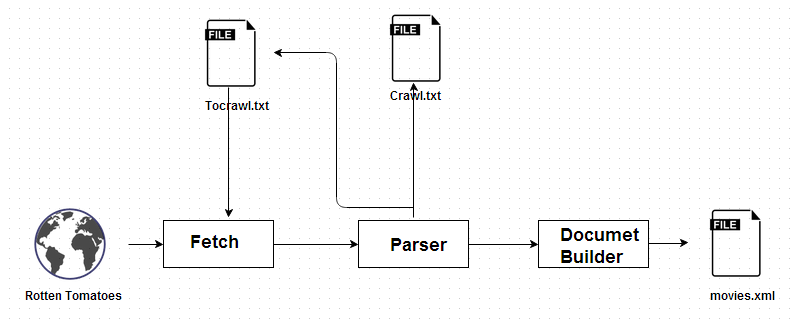
\includegraphics[width=4.0in]{crawler_arch.png}
    \caption{Crawler Architecture}
    \label{fig:architecture}
\end{figure}

\subsubsection{Challenges}
The main challenge was to encounter the non uniformity of the content in Rotten Tomatoes web pages. Some of the web pages contained all the information about the movies while in others, a few of the information fields were missing. The crawler was designed to scrap the HTML data in a way such that maximum amount of information can be retrieved. Another challenge was to make sure that the crawler is not blocked by the site. This was handled by building the crawler in a flexible way so that, during an iteration, the crawler will only crawl through a specific number of pages specified to it as a parameter. After each iteration, the URLs which are already crawlled and the URLs those are yet to be crawlled are written back to \textit{Crawl.txt} and \textit{Tocrawl.txt} respectively which will be used in the next iterations. Fig.\ref{fig:xmlFile} shows an entry in the \textit{movies.xml} file.

\begin{figure}[H]
    \centering
    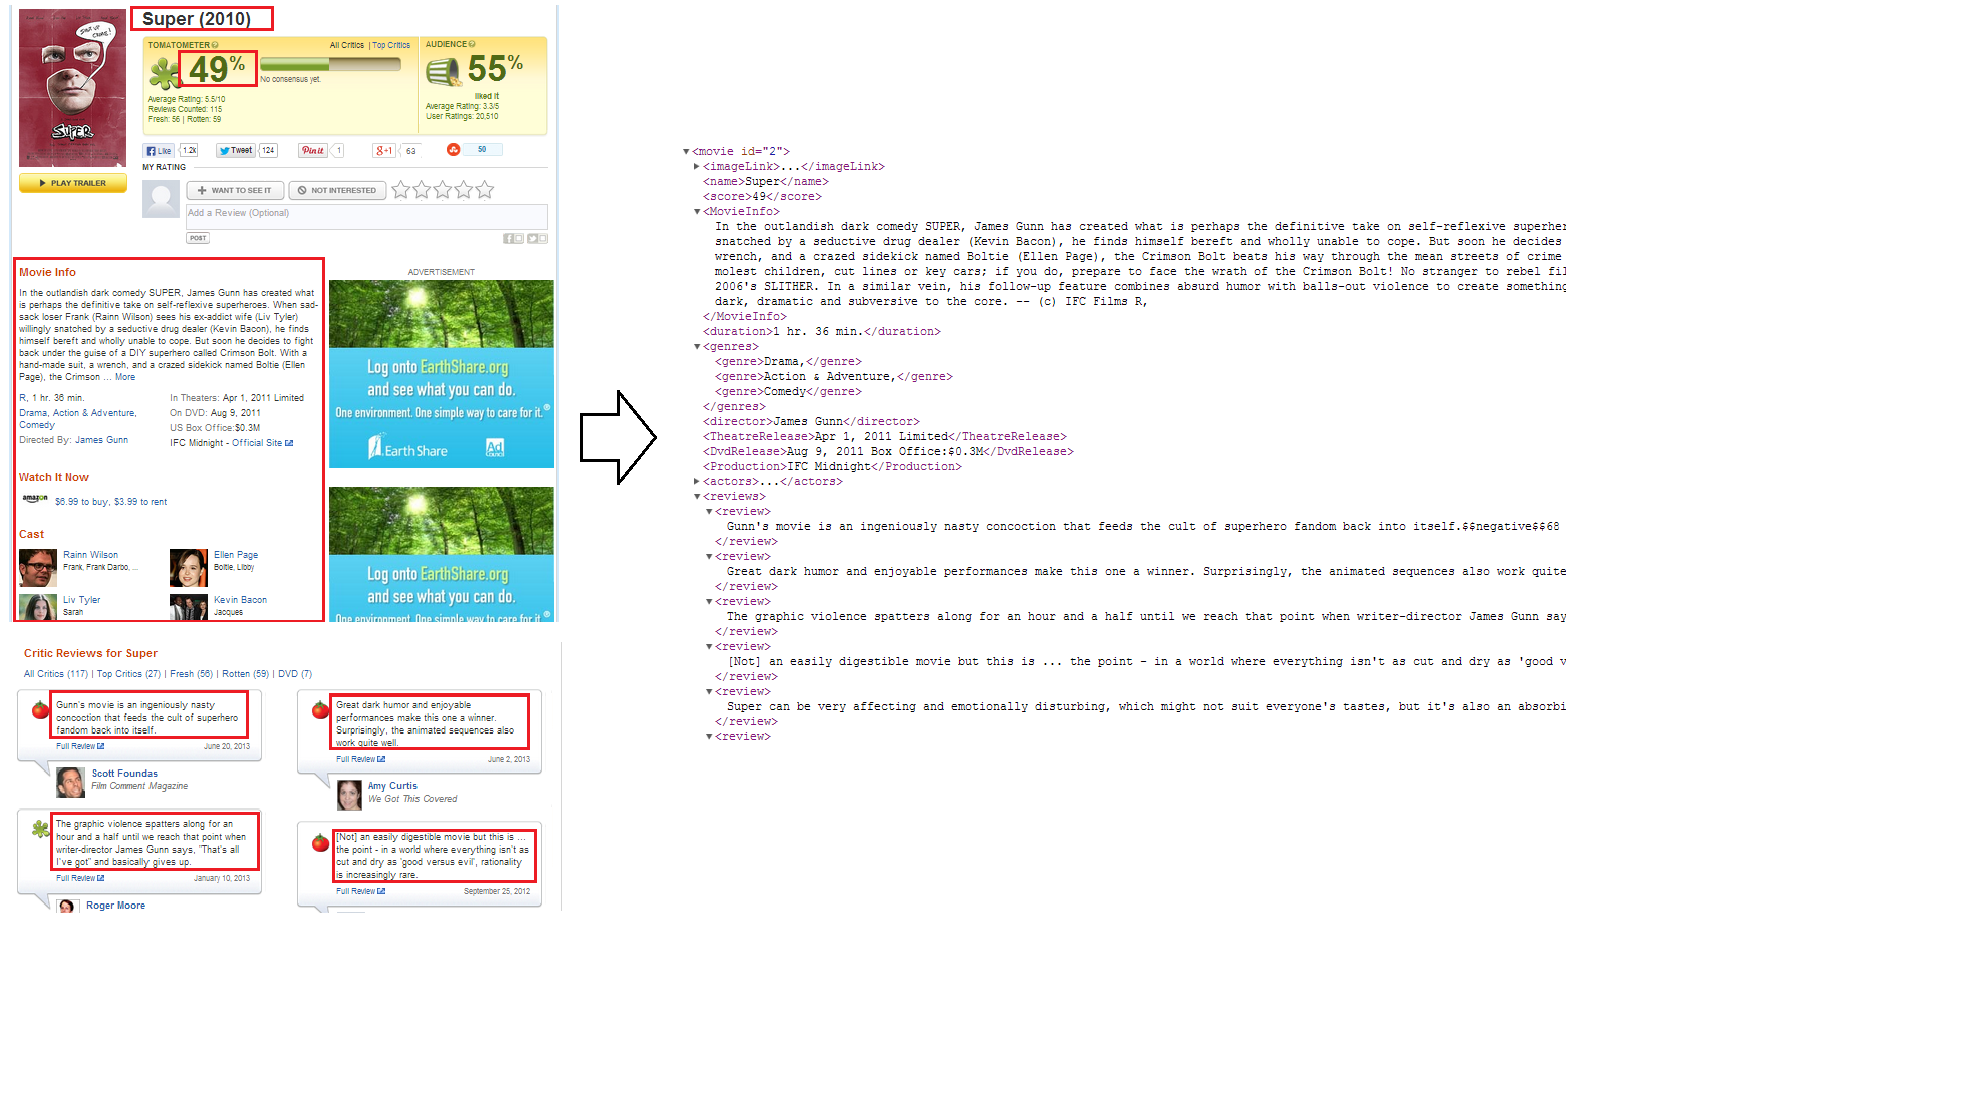
\includegraphics[width=4.5in]{rot.png}
    \caption{Collecting data from Rotten Tomatoes}
    \label{fig:xmlFile}
\end{figure}

\subsubsection{Evaluation \& Summary}
After several iterations, we collected 6227 movies each containing movie metadata and the reviews. We collected only top critics reviews because we feel that those are the most representative of all the reviews. As focused crawler parse all the content in documents and filter only the relevant content for the application, crawling took more time than a normal crawler would take. But the flexibility in the design of the crawler allowed us to run it in iterations so we did not face any issue regarding the time for crawling. We took 20 random samples from the file and compared the contents with the content in the site. In all the cases, we were able to capture all the relevant data needed for the search and sentiment analysis functionality.

\subsection{Lucene Search, Wildcard Queries \& Autocomplete : S.R. Patra}
\subsubsection{Motivation}
Lucene provides very rich library functions to implement indexing and search. So we implemented lucene search as a metric to evaluate our boolean and vector space model performances. 
\subsubsection{Approach}
Lucene.net library was used for generating the index and for getting the search results from the processed query. We limited our search results to be 10 top relevant results. Index was created for different fields to allow the user to search based on any criteria they want i.e. based on actor, director, genres etc. We also implemented the \textit{Autocomplete} feature to help the user with the query. This feature was developed in \textit{JQuery} and was implemented as a web service which queries the database about possible movie names after each input letter in the text box. 

\paragraph{}
Wild card queries were used to provide query suggestions to the user when the user only knows parts of the terms in the query. The speech to text query assistance feature was also included using the HTML5 Webkit speech. All the features discussed above are shown in fig.\ref{fig:search}.
\begin{figure}[H]
    \centering
    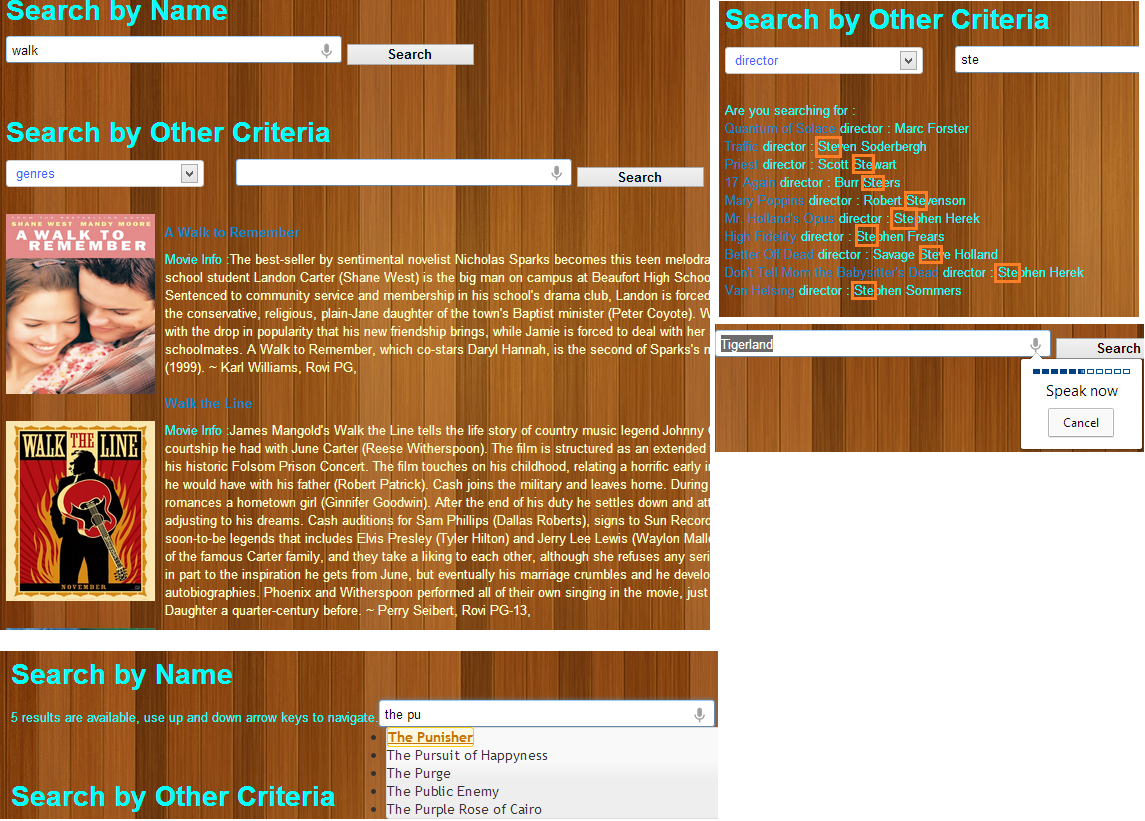
\includegraphics[width=4.5in]{search.png}
    \caption{Searching functionalities}
    \label{fig:search}
\end{figure}

\subsubsection{Evaluation \& Summary}
After trying a number of sample queries for different search criterias, we feel that the search provided quite relevant results in all the cases. The wildcard queries were also accurate in their suggestions and the users were able to retrieve relevant movie names based on parts of the search query terms. 
\subsection{Tf-idf: F.N. Butnariu}
\subsubsection{Motivation}
Initially the tf-idf component was developed to primarily support the vector space model, but subsequently it became obvious that it will also play an important role in the hierarchical agglomerative clustering task, where cosine similarity was employed to measure resemblance of movies based on information such as title, description, genre, director and cast.

Considering our dataset of movies in this task we aimed to assign a tf-idf weight to each term in each document pertaining information about a movie. The input may be viewed as a collection of documents, where a document contains metadata about a single movie such as title, description, genre, director, cast, reviews and other details. The output is a set of triples \verb+<term, ID, weight>+, where \verb+ID+ identifies a document in our collection in which \verb+term+ has a tf-idf value given by \verb+weight+.

\subsubsection{Approach}

The entire information about our set of movies resides in a single XML file, so the first challenge was to transpose this information into a document representation corresponding to each movie in our dataset. This was accomplished using a SAX parser, which basically created for each movie a String to which all the relevant information about the movie was appended. Therefore, at this stage each document pertaining information about a movie can be viewed as a large String. In the next stage by employing one of Lucene's text analyzers each String corresponding to a movie was tokenized into a bag of words. We do not take into account the order of the words within a document, but instead only consider the number of occurrences of a word inside a document. Here we use $term$ and $word$ interchangeably.

At the heart of the tf-idf component lies an index having the structure represented in Listing~\ref{lst:tf-idf-index}. The index records for each term its document frequency, i.e. the number of documents in our collection in which term occurs. In addition, for each term a list of pairs \verb+<ID>, <term frequency>+ is stored. For every document identified by \verb+ID+, in which the term is present, there is a corresponding term frequency, i.e. the number of occurrences of the term inside the document.

\begin{lstlisting}[caption={The structure of the tf-idf index},label={lst:tf-idf-index}]
<term>, <document frequency>:
	(<ID>, <term frequency>;
	<ID>, <term frequency>;
	...
	<ID>, <term frequency>; ...)
<term>, <document frequency>:
	(<ID>, <term frequency>;
	<ID>, <term frequency>;
	...
	<ID>, <term frequency>; ...)
\end{lstlisting}

This index was built by going over each document in our collection in one pass and examining each term within a document. Thus it also functions as a dictionary since it encompasses all the terms found in our document collection. 

By making use of this index a tf-idf weight can quickly be calculated using Equation~\ref{eq:tf-idf}.

\begin{equation}
\label{eq:tf-idf}
tfidf_{t,d} = tf_{t,d} \times log\frac{N}{df_t}
\end{equation}

The set of triples \verb+<term, ID, weight>+ can be computed by going over the entire index in one pass.

\subsubsection{Argumentation for choice}

Parsing the XML file holding our dataset of movies presented us with two options, namely, either using a SAX parser or a DOM parser. We opted to employ the former approach because of its reduced memory overhead in comparison with the latter technique, which would load in memory a costly tree data structure for the entire XML file.

Following the same line of reducing memory overhead and keeping in mind that in-memory operations are much faster than disk access operations, we decided to use the index described earlier to compute tf-idf weights on the fly instead of relying on a much larger data structure, which would have hold for every possible term and for every possible document a tf-idf weight.

Although the tf-idf weighting scheme is designed to assign a low weight to terms appearing in almost all documents, we opted to leave out stop words in most of the cases.

\subsubsection{Evaluation of obtained results}

\subsubsection{Conclusions}



\section{Machine Learning}

\section{Conclusion}
\input{conclusion.tex}
\end{document}